\experiment{Infix Postfix Conversions}{25/10/2023}

\section{Aim}
Write a menu driven C Program, to do the following operations using a stack data structure:
\\a. Convert an infix expression to a postfix expression
\\b. Evaluate the postfix expression

\section{Algorithm}
 {\fontfamily{lmtt}\selectfont

  \subsection{Infix to Postfix Conversion}
  Create a function \texttt{infixToPostfix(infix, s)}:
  \begin{enumerate}[label=\arabic*:,left=0pt]
    \item \textbf{Start}
    \item Initialize \texttt{j} to the length of \texttt{infix}.
    \item Append ')' to the end of \texttt{infix}.
    \item Loop through each character \texttt{infix[i]}:
          \begin{enumerate}[label=2.\arabic*.]
            \item If \texttt{infix[i]} is an operand, print it.
            \item If \texttt{infix[i]} is '(', push it onto the stack.
            \item If \texttt{infix[i]} is ')':
                  \begin{enumerate}[label=2.3.\arabic*.]
                    \item Pop and print elements from the stack until '(' is encountered.
                    \item Pop '(' from the stack.
                  \end{enumerate}
            \item If \texttt{infix[i]} is an operator:
                  \begin{enumerate}[label=2.4.\arabic*.]
                    \item While stack is not empty and the priority of \texttt{infix[i]} is less than or equal \newline to the priority of the top element of the stack, pop and print from the stack.
                    \item Push \texttt{infix[i]} onto the stack.
                  \end{enumerate}
          \end{enumerate}
    \item \textbf{Stop}
  \end{enumerate}

  \subsection{Postfix Evaluation}
  Create a function \texttt{postfixEvaluate(postfix, s)}:
  \begin{enumerate}[label=\arabic*:,left=0pt]
    \item \textbf{Start}
    \item Initialize \texttt{j} to the length of \texttt{postfix}.
    \item Loop through each character \texttt{postfix[i]}:
          \begin{enumerate}[label=2.\arabic*.]
            \item If \texttt{postfix[i]} is an operand, push its numeric value onto the stack.
            \item If \texttt{postfix[i]} is an operator:
                  \begin{enumerate}[label=2.2.\arabic*.]
                    \item Pop two operands (\texttt{a} and \texttt{b}) from the stack.
                    \item Perform the operation (\texttt{a} \texttt{postfix[i]} \texttt{b}).
                    \item Push the result onto the stack.
                  \end{enumerate}
            \item Print the top element of the stack as the final result.
          \end{enumerate}
    \item \textbf{Stop}
  \end{enumerate}

  \subsection{Get Priority Function}
  Create a function \texttt{getPriority(op)}:
  \begin{enumerate}[label=\arabic*:,left=0pt]
    \item \textbf{Start}
    \item If \texttt{op} is '(', return 0.
    \item If \texttt{op} is '+' or '-', return 1.
    \item If \texttt{op} is '*' or '/', return 2.
    \item If \texttt{op} is '\textasciicircum', return 3.
    \item \textbf{Stop}
  \end{enumerate}

  \subsection{Main Function}
  In the \texttt{main} function:
  \begin{enumerate}[label=\arabic*:, start=1]
    \item \textbf{Start}
    \item Take user input for the expression \texttt{exp}.
    \item Create a stack \texttt{s} using \texttt{createStack()}.
    \item Take user input for the choice \texttt{ch} (1 for infix to postfix, 2 for postfix evaluate).
    \item If \texttt{ch} is 1, call \texttt{infixToPostfix(exp, s)}.
    \item If \texttt{ch} is 2, call \texttt{postfixEvaluate(exp, s)}.
    \item If \texttt{ch} is neither 1 nor 2, print "Invalid choice".
    \item \textbf{Stop}
  \end{enumerate}
 }
\newblock
\section{C Program}
\begin{lstlisting}[label={list:c_program:infix-postfix}]
#include <stdio.h>
#include <stdlib.h>

typedef struct stack
{
  int top;
  int size;
  int arr[100];
} stack;

stack *createStack();
void push(stack *s, int data);
void pop(stack *s);
void infixToPostfix(char *infix, stack *s);
void postfixToInfix(char *postfix, stack *s);
int getPriority(char op);

int main()
{
  printf("\nEnter the expression: ");
  char exp[100];
  gets(exp);
  stack *s = createStack();
  printf("1)infix to postfix\n2)postfix evaluate\nChoice: ");
  int ch;
  scanf("%d", &ch);
  if (ch == 1)
  {
    infixToPostfix(exp, s);
  }
  else if (ch == 2)
  {
    postfixEvaluate(exp, s);
  }
  else
  {
    printf("Invalid choice\n");
  }
}

void infixToPostfix(char *infix, stack *s)
{
  int j = 0;
  for (j = 0; infix[j] != '\0'; j++)
    ;
  infix[j] = ')';
  for (int i = 0; i <= j; i++)
  {
    if (infix[i] >= 'a' && infix[i] <= 'z')
    {
      printf("%c", infix[i]);
    }
    else if (infix[i] == '(')
    {
      push(s, infix[i]);
    }
    else if (infix[i] == ')')
    {
      while (s->top >= 0 && s->arr[s->top] != '(')
      {
        printf("%c", s->arr[s->top]);
        pop(s);
      }
      if (s->top >= 0)
        pop(s);
    }
    else
    {
      while(s->top >= 0 && getPriority(infix[i]) <= getPriority(s->arr[s->top])){
          printf("%c", s->arr[s->top]);
          pop(s);
      }
      push(s, infix[i]);
    }
  }
}

void postfixEvaluate(char *postfix, stack *s)
{
  int j = 0;
  for (j = 0; postfix[j] != '\0'; j++)
    ;

  for (int i = 0; i < j; i++)
  {
    printf("%c", postfix[i]);
  }
  for (int i = 0; i < j; i++)
  {
    int c = postfix[i] - '0';
    if (postfix[i] == ' ')
      continue;
    if (c >= 0 && c <= 9)
    {
      int val = 0;
      while (i < j && postfix[i] >= '0' && postfix[i] <= '9')
      {
        val = val * 10 + (postfix[i] - '0');
        i++;
      }
      i--;
      push(s, val);
    }
    else
    {
      int a = s->arr[s->top];
      pop(s);
      int b = s->arr[s->top];
      pop(s);
      if (postfix[i] == '+')
      {
        push(s, a + b);
      }
      else if (postfix[i] == '-')
      {
        push(s, b - a);
      }
      else if (postfix[i] == '*')
      {
        push(s, a * b);
      }
      else if (postfix[i] == '/')
      {
        push(s, b / a);
      }
      else
      {
        printf("Invalid character\n");
        return;
      }
    }
  }
  printf("\nExpression = %d\n", s->arr[s->top]);
}

int getPriority(char op)
{
  switch(op)
  {
    case '(':
      return 0;
      break;
    case '+': 
      return 1;
      break;
    case '-': 
      return 1;
      break;
    case '*': 
      return 2;
      break;
    case '/': 
      return 2;
      break;
    case '^': 
      return 3;
      break;
  }
}

stack *createStack()
{
  stack *s = (stack *)malloc(sizeof(stack));
  s->top = -1;
  s->size = 100;
  return s;
}

void push(stack *s, int data)
{
  if (s->top == s->size - 1)
  {
    printf("Stack Overflow\n");
    return;
  }
  s->top++;
  s->arr[s->top] = data;
}

void pop(stack *s)
{
  if (s->top < 0)
  {
    printf("Stack Underflow\n");
    return;
  }
  s->top--;
}
\end{lstlisting}

\section{Output}
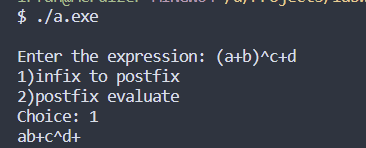
\includegraphics[]{Cycle_1/Outputs/infixpostfix1.png}
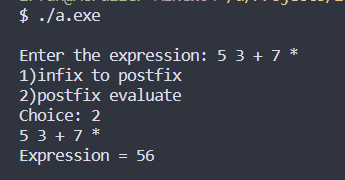
\includegraphics[]{Cycle_1/Outputs/infixpostfix2.png}

\section{Result}
Infix expression converted to postfix and postfix expression evaluated. The program was
executed and output verified.